% Options for packages loaded elsewhere
\PassOptionsToPackage{unicode}{hyperref}
\PassOptionsToPackage{hyphens}{url}
\PassOptionsToPackage{dvipsnames,svgnames,x11names}{xcolor}
%
\documentclass[
  title=normal,
  notoc,
  bib=normal]{mnye}
\usepackage{amsmath,amssymb}
\usepackage{lmodern}
\usepackage{iftex}
\ifPDFTeX
  \usepackage[T1]{fontenc}
  \usepackage[utf8]{inputenc}
  \usepackage{textcomp} % provide euro and other symbols
\else % if luatex or xetex
  \usepackage{unicode-math}
  \defaultfontfeatures{Scale=MatchLowercase}
  \defaultfontfeatures[\rmfamily]{Ligatures=TeX,Scale=1}
\fi
% Use upquote if available, for straight quotes in verbatim environments
\IfFileExists{upquote.sty}{\usepackage{upquote}}{}
\IfFileExists{microtype.sty}{% use microtype if available
  \usepackage[]{microtype}
  \UseMicrotypeSet[protrusion]{basicmath} % disable protrusion for tt fonts
}{}
\makeatletter
\@ifundefined{KOMAClassName}{% if non-KOMA class
  \IfFileExists{parskip.sty}{%
    \usepackage{parskip}
  }{% else
    \setlength{\parindent}{0pt}
    \setlength{\parskip}{6pt plus 2pt minus 1pt}}
}{% if KOMA class
  \KOMAoptions{parskip=half}}
\makeatother
\usepackage{xcolor}
\IfFileExists{xurl.sty}{\usepackage{xurl}}{} % add URL line breaks if available
\IfFileExists{bookmark.sty}{\usepackage{bookmark}}{\usepackage{hyperref}}
\hypersetup{
  pdftitle={Instalación de R y RStudio},
  pdfauthor={Eva María Mazcuñán Navarro},
  colorlinks=true,
  linkcolor={Maroon},
  filecolor={Maroon},
  citecolor={Blue},
  urlcolor={Blue},
  pdfcreator={LaTeX via pandoc}}
\urlstyle{same} % disable monospaced font for URLs
\usepackage{color}
\usepackage{fancyvrb}
\newcommand{\VerbBar}{|}
\newcommand{\VERB}{\Verb[commandchars=\\\{\}]}
\DefineVerbatimEnvironment{Highlighting}{Verbatim}{commandchars=\\\{\}}
% Add ',fontsize=\small' for more characters per line
\usepackage{framed}
\definecolor{shadecolor}{RGB}{248,248,248}
\newenvironment{Shaded}{\begin{snugshade}}{\end{snugshade}}
\newcommand{\AlertTok}[1]{\textcolor[rgb]{0.94,0.16,0.16}{#1}}
\newcommand{\AnnotationTok}[1]{\textcolor[rgb]{0.56,0.35,0.01}{\textbf{\textit{#1}}}}
\newcommand{\AttributeTok}[1]{\textcolor[rgb]{0.77,0.63,0.00}{#1}}
\newcommand{\BaseNTok}[1]{\textcolor[rgb]{0.00,0.00,0.81}{#1}}
\newcommand{\BuiltInTok}[1]{#1}
\newcommand{\CharTok}[1]{\textcolor[rgb]{0.31,0.60,0.02}{#1}}
\newcommand{\CommentTok}[1]{\textcolor[rgb]{0.56,0.35,0.01}{\textit{#1}}}
\newcommand{\CommentVarTok}[1]{\textcolor[rgb]{0.56,0.35,0.01}{\textbf{\textit{#1}}}}
\newcommand{\ConstantTok}[1]{\textcolor[rgb]{0.00,0.00,0.00}{#1}}
\newcommand{\ControlFlowTok}[1]{\textcolor[rgb]{0.13,0.29,0.53}{\textbf{#1}}}
\newcommand{\DataTypeTok}[1]{\textcolor[rgb]{0.13,0.29,0.53}{#1}}
\newcommand{\DecValTok}[1]{\textcolor[rgb]{0.00,0.00,0.81}{#1}}
\newcommand{\DocumentationTok}[1]{\textcolor[rgb]{0.56,0.35,0.01}{\textbf{\textit{#1}}}}
\newcommand{\ErrorTok}[1]{\textcolor[rgb]{0.64,0.00,0.00}{\textbf{#1}}}
\newcommand{\ExtensionTok}[1]{#1}
\newcommand{\FloatTok}[1]{\textcolor[rgb]{0.00,0.00,0.81}{#1}}
\newcommand{\FunctionTok}[1]{\textcolor[rgb]{0.00,0.00,0.00}{#1}}
\newcommand{\ImportTok}[1]{#1}
\newcommand{\InformationTok}[1]{\textcolor[rgb]{0.56,0.35,0.01}{\textbf{\textit{#1}}}}
\newcommand{\KeywordTok}[1]{\textcolor[rgb]{0.13,0.29,0.53}{\textbf{#1}}}
\newcommand{\NormalTok}[1]{#1}
\newcommand{\OperatorTok}[1]{\textcolor[rgb]{0.81,0.36,0.00}{\textbf{#1}}}
\newcommand{\OtherTok}[1]{\textcolor[rgb]{0.56,0.35,0.01}{#1}}
\newcommand{\PreprocessorTok}[1]{\textcolor[rgb]{0.56,0.35,0.01}{\textit{#1}}}
\newcommand{\RegionMarkerTok}[1]{#1}
\newcommand{\SpecialCharTok}[1]{\textcolor[rgb]{0.00,0.00,0.00}{#1}}
\newcommand{\SpecialStringTok}[1]{\textcolor[rgb]{0.31,0.60,0.02}{#1}}
\newcommand{\StringTok}[1]{\textcolor[rgb]{0.31,0.60,0.02}{#1}}
\newcommand{\VariableTok}[1]{\textcolor[rgb]{0.00,0.00,0.00}{#1}}
\newcommand{\VerbatimStringTok}[1]{\textcolor[rgb]{0.31,0.60,0.02}{#1}}
\newcommand{\WarningTok}[1]{\textcolor[rgb]{0.56,0.35,0.01}{\textbf{\textit{#1}}}}
\usepackage{longtable,booktabs,array}
\usepackage{calc} % for calculating minipage widths
% Correct order of tables after \paragraph or \subparagraph
\usepackage{etoolbox}
\makeatletter
\patchcmd\longtable{\par}{\if@noskipsec\mbox{}\fi\par}{}{}
\makeatother
% Allow footnotes in longtable head/foot
\IfFileExists{footnotehyper.sty}{\usepackage{footnotehyper}}{\usepackage{footnote}}
\makesavenoteenv{longtable}
\usepackage{graphicx}
\makeatletter
\def\maxwidth{\ifdim\Gin@nat@width>\linewidth\linewidth\else\Gin@nat@width\fi}
\def\maxheight{\ifdim\Gin@nat@height>\textheight\textheight\else\Gin@nat@height\fi}
\makeatother
% Scale images if necessary, so that they will not overflow the page
% margins by default, and it is still possible to overwrite the defaults
% using explicit options in \includegraphics[width, height, ...]{}
\setkeys{Gin}{width=\maxwidth,height=\maxheight,keepaspectratio}
% Set default figure placement to htbp
\makeatletter
\def\fps@figure{htbp}
\makeatother
\setlength{\emergencystretch}{3em} % prevent overfull lines
\providecommand{\tightlist}{%
  \setlength{\itemsep}{0pt}\setlength{\parskip}{0pt}}
\setcounter{secnumdepth}{5}
\usepackage{ehyperref}
\colorlet{etoccolor}{greenlink}
% This file is created the first time epdf_document is invoked
% but will not be overwriten afterwards.
%
% Preamble
\degree{mecinf}
\term{2021-2022}
\ifLuaTeX
  \usepackage{selnolig}  % disable illegal ligatures
\fi
\usepackage[]{biblatex}

\title{Instalación de R y RStudio}
\author{Eva María Mazcuñán Navarro}
\date{}

\begin{document}
\maketitle

% This file is created the first time epdf_document is invoked
% but will not be overwriten afterwards.
%
% Before Body

{
\hypersetup{linkcolor=etoccolor}
\setcounter{tocdepth}{2}
\tableofcontents
}
\hypertarget{section}{%
\section*{}\label{section}}

Utilizaremos el lenguaje \textsf{R}, vía \textsf{RStudio}, para realizar las prácticas y resolver las tareas que se plantearán en la asignatura.

\begin{center}
\includegraphics[width=0.1\linewidth]{images/r-logo} 
\includegraphics[width=0.3\linewidth]{images/rstudio-logo} \end{center}

\begin{figure}

{\centering \includegraphics[width=0.33\linewidth]{https://www.fairvote.ca/wp-content/uploads/2019/12/Western-alienation-website-FPTP-page} \includegraphics[width=0.33\linewidth]{https://www.fairvote.ca/wp-content/uploads/2019/12/Toronto-Peel-halton-2019-results-website-FPTP} 

}

\caption{Examples of the FPTP bias: In Prairies (left) and Greater Toronto area (right). Source: www.fairvote.ca}\label{fig:unnamed-chunk-2}
\end{figure}

En este documento encontrarás las instrucciones para instalar \textsf{R} y \textsf{RStudio} en tu equipo.

Utiliza la tabla de contenidos del panel izquierdo para elegir el sistema operativo donde quieres realizar la instalación, y sigue los pasos que se describen allí.

\hypertarget{linux}{%
\section{Linux}\label{linux}}

\begin{center}
\includegraphics[width=0.15\linewidth]{images/os/tux-flat} \end{center}

\hypertarget{instalaciuxf3n-de-r}{%
\subsection{Instalación de R}\label{instalaciuxf3n-de-r}}

En este apartado se describen las instrucciones para instalar R en Ubuntu. Para otras distribuciones de Linux consulta \href{https://ftp.cixug.es/CRAN/bin/linux/}{este link}.

\begin{center}
\includegraphics[width=0.15\linewidth]{images/os/ubuntu} \end{center}

Para instalar R en Ubuntu necesitamos instalar los paquetes \texttt{r-base} y \texttt{r-base-dev}. Siguiendo los siguientes pasos obtendrás las versiones más recientes y recibirás las últimas actualizaciones.

\textbf{PASO 1: } Actualizar los índices:

\begin{Shaded}
\begin{Highlighting}[]
\FunctionTok{sudo}\NormalTok{ apt update }
\end{Highlighting}
\end{Shaded}

\textbf{PASO 2: } Instalar un par de paquetes auxiliares:

\begin{Shaded}
\begin{Highlighting}[]
\FunctionTok{sudo}\NormalTok{ apt install }\AttributeTok{{-}{-}no{-}install{-}recommends}\NormalTok{ software{-}properties{-}common dirmngr }
\end{Highlighting}
\end{Shaded}

\textbf{PASO 3: } Añadir la clave para el repositorio que añadiremos en el siguiente paso (por Michael Rutter):

\begin{Shaded}
\begin{Highlighting}[]
\FunctionTok{wget} \AttributeTok{{-}qO{-}}\NormalTok{ https://cloud.r{-}project.org/bin/linux/ubuntu/marutter\_pubkey.asc }\KeywordTok{|} \FunctionTok{sudo}\NormalTok{ tee }\AttributeTok{{-}a}\NormalTok{ /etc/apt/trusted.gpg.d/cran\_ubuntu\_key.asc}
\end{Highlighting}
\end{Shaded}

\textbf{PASO 4: } Añadir repositorio (de \href{https://cran.r-project.org/}{CRAN}):

\begin{Shaded}
\begin{Highlighting}[]
\FunctionTok{sudo}\NormalTok{ add{-}apt{-}repository }\StringTok{"deb https://cloud.r{-}project.org/bin/linux/ubuntu }\VariableTok{$(}\ExtensionTok{lsb\_release} \AttributeTok{{-}cs}\VariableTok{)}\StringTok{{-}cran40/"}
\end{Highlighting}
\end{Shaded}

\textbf{PASO 5: } Volver a actualizar los índices:

\begin{Shaded}
\begin{Highlighting}[]
\FunctionTok{sudo}\NormalTok{ apt update }
\end{Highlighting}
\end{Shaded}

\textbf{PASO 6: } Instalar \texttt{r-base} y \texttt{r-base-dev}:

\begin{Shaded}
\begin{Highlighting}[]
\FunctionTok{sudo}\NormalTok{ apt install }\AttributeTok{{-}{-}no{-}install{-}recommends}\NormalTok{ r{-}base r{-}base{-}dev }
\end{Highlighting}
\end{Shaded}

\hypertarget{instalaciuxf3n-de-rstudio}{%
\subsection{Instalación de RStudio}\label{instalaciuxf3n-de-rstudio}}

Una vez instalado R, sigue los siguientes pasos para instalar RStudio.

\textbf{PASO 1: }
Accede a la página de descargas de RStudio pinchando \href{https://rstudio.com/products/rstudio/download/\#download}{aquí}.

En el apartado \textbf{All Installers} descarga el instalador más reciente para tu versión (para Ubuntu 20, descarga Ubuntu 18/Debian 10, ver imagen debajo).

\begin{figure}

{\centering 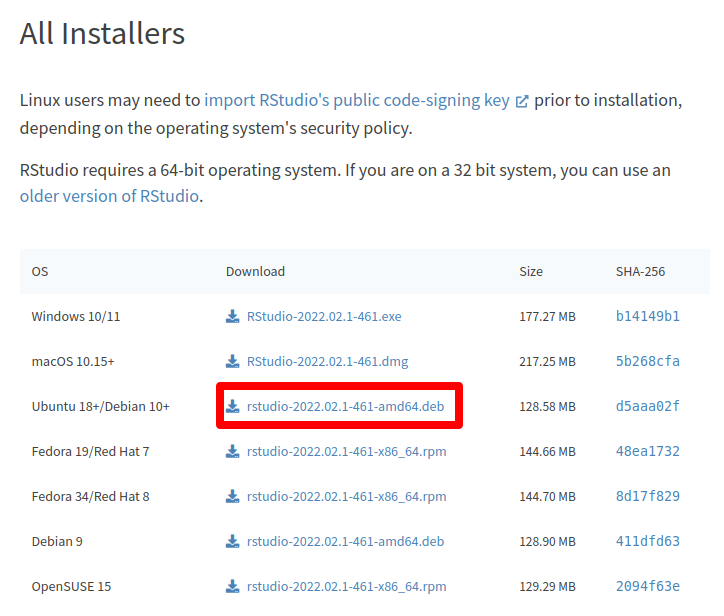
\includegraphics[width=0.9\linewidth]{images/rstudio-ubuntu} 

}

\caption{Página de descargas de RStudio}\label{fig:unnamed-chunk-11}
\end{figure}

\textbf{PASO 2: }
Cuando se complete la descarga del paso anterior, haz doble click en el archivo \texttt{.deb} descargado. Se abrirá con el gestor de software de Ubuntu. Presiona el botón `Instalar' para terminar.

\hypertarget{windows}{%
\section{Windows}\label{windows}}

\begin{center}
\includegraphics[width=0.15\linewidth]{images/os/windows} \end{center}

A continuación se proporcionan los links para la descarga de los instaladores de R y RStudio en Windows. En ambos casos, se descargará un archivo ejecutable que gestionará la instalación de R / RStudio en tu equipo.

Puedes conservar todas las opciones de instalación que aparecen por defecto.

\hypertarget{instalaciuxf3n-de-r-1}{%
\subsection{Instalación de R}\label{instalaciuxf3n-de-r-1}}

Accede a la página de descargas de R para Windows pinchando \href{https://cloud.r-project.org/bin/windows/base/}{aquí}, y haz click el link de título `Download R 4.2.0 for Windows', que encontrarás al principio de la página (ver imagen debajo).

\begin{figure}

{\centering 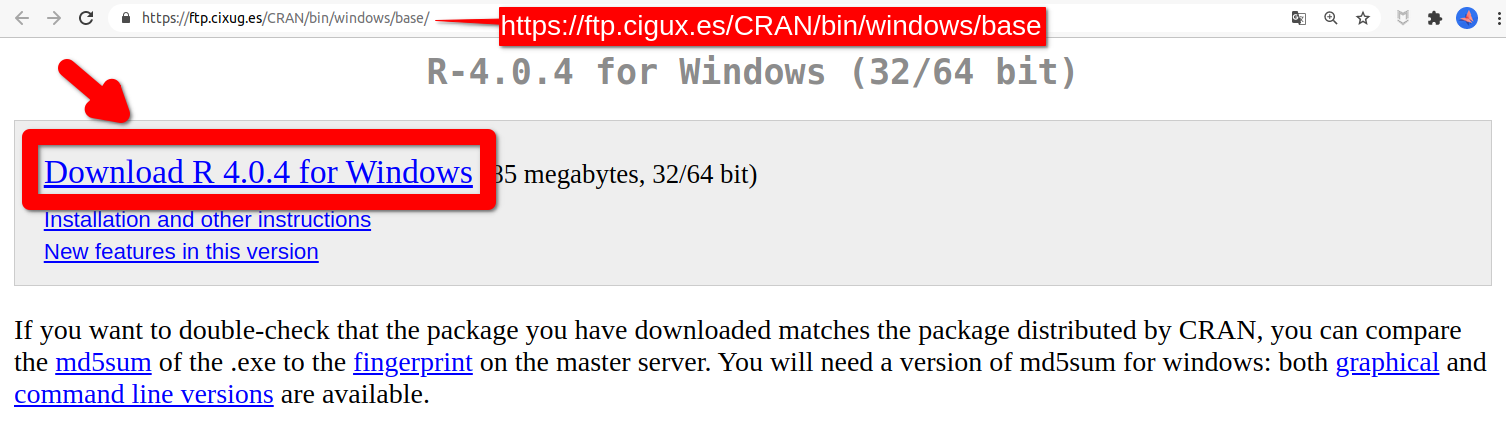
\includegraphics[width=0.65\linewidth]{images/r-windows} 

}

\caption{Página de descargas de R para Windows}\label{fig:unnamed-chunk-13}
\end{figure}

\hypertarget{instalaciuxf3n-de-rstudio-1}{%
\subsection{Instalación de RStudio}\label{instalaciuxf3n-de-rstudio-1}}

Accede a la página de descargas de RStudio pinchando \href{https://rstudio.com/products/rstudio/download/\#download}{aquí}, y, en la tabla del apartado \textbf{All Installers}, haz click en el link de descarga correspondiente a Windows 10/11 (ver imagen).

\begin{figure}

{\centering 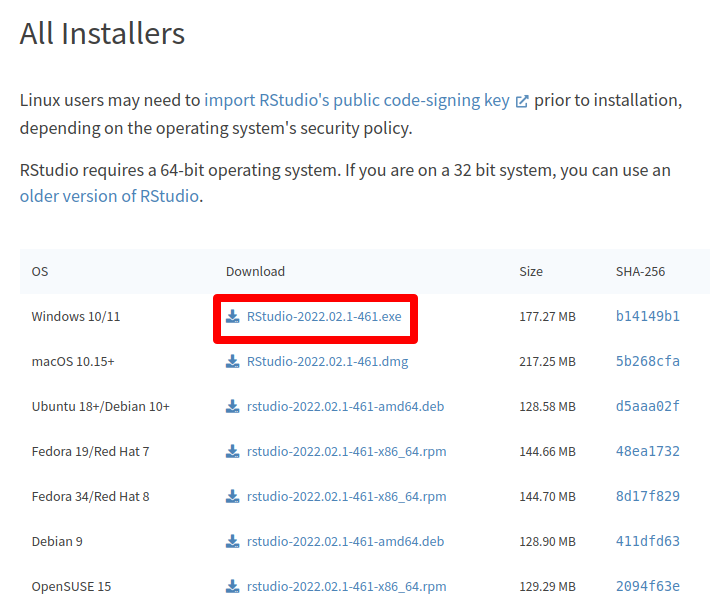
\includegraphics[width=0.9\linewidth]{images/rstudio-windows} 

}

\caption{Página de descargas de RStudio}\label{fig:unnamed-chunk-14}
\end{figure}

\hypertarget{mac}{%
\section{Mac OS X}\label{mac}}

\begin{center}
\includegraphics[width=0.15\linewidth]{images/os/apple} \end{center}

\hypertarget{instalaciuxf3n-de-r-2}{%
\subsection{Instalación de R}\label{instalaciuxf3n-de-r-2}}

Accede a la página de descargas de \textsf{R} para Mac OS X pinchando \href{https://cloud.r-project.org/bin/macosx/}{aquí} y descarga el instalador correspondiente a la versión de tu equipo (ver imagen).

\begin{figure}

{\centering 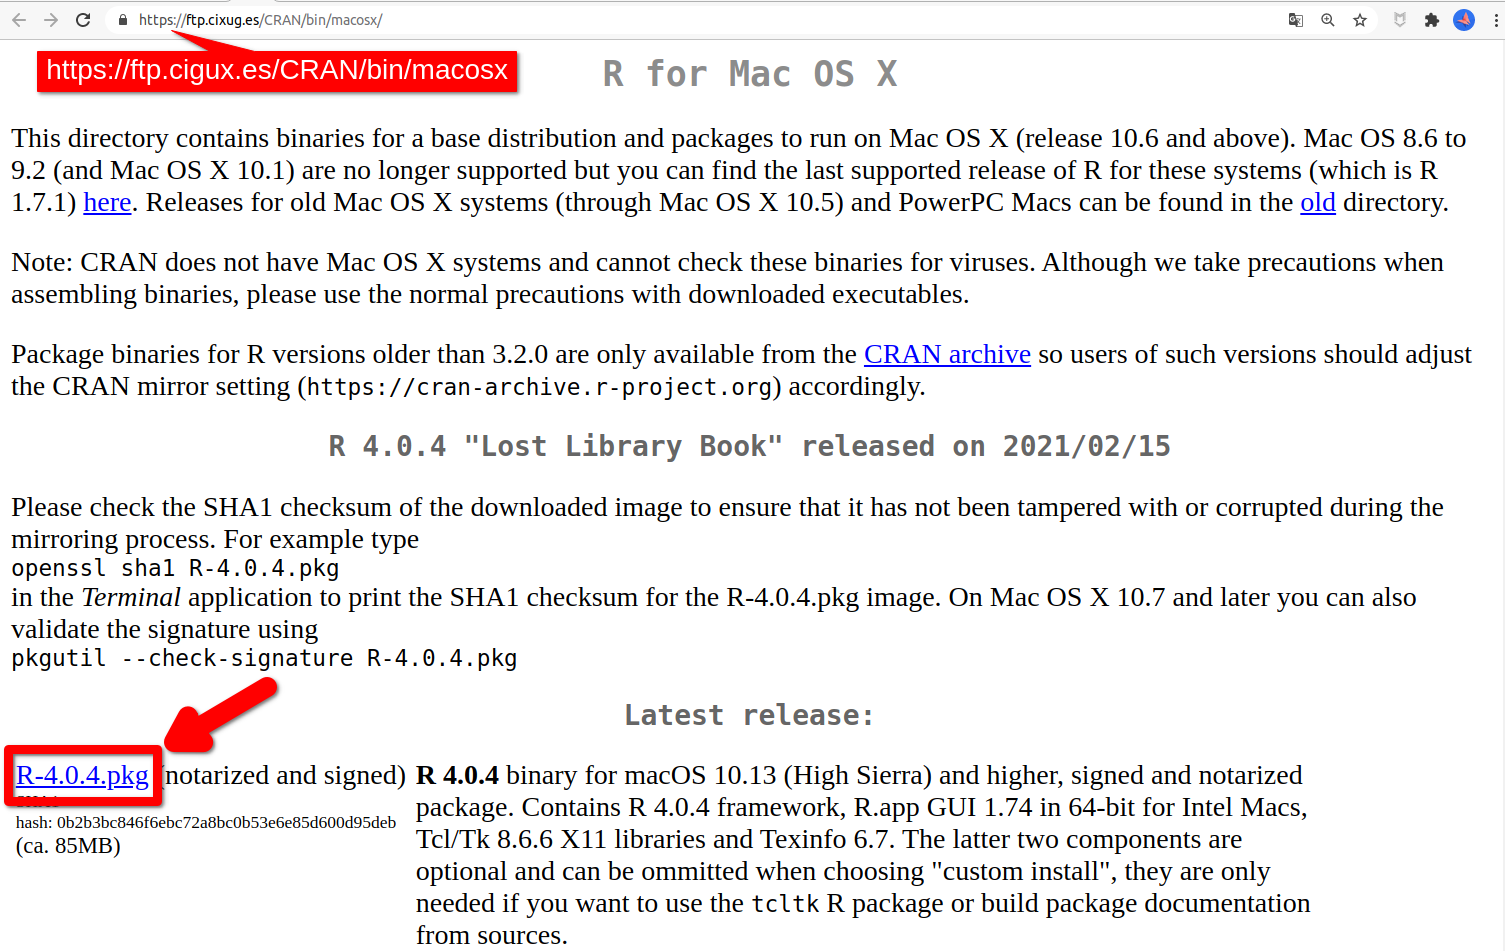
\includegraphics[width=1\linewidth]{images/r-mac} 

}

\caption{Página de descargas de R para Mac}\label{fig:unnamed-chunk-16}
\end{figure}

Solo tienes que ejecutar el archivo \texttt{pgk} que se descargará para instalar R en tu equipo. Puedes conservar todas las opciones de instalación por defecto.

\hypertarget{instalaciuxf3n-de-rstudio-2}{%
\subsection{Instalación de RStudio}\label{instalaciuxf3n-de-rstudio-2}}

Accede a la página de descargas de RStudio pinchando \href{https://rstudio.com/products/rstudio/download/\#download}{aquí}, y, en la tabla del apartado \textbf{All Installers}, haz click en el link de descarga correspondiente a macOS 10.15+ (ver imagen debajo).

\begin{figure}

{\centering 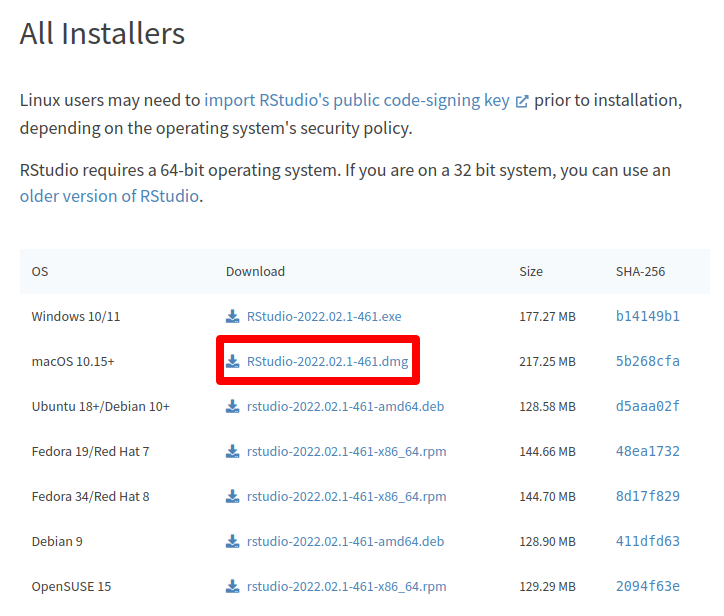
\includegraphics[width=0.9\linewidth]{images/rstudio-mac} 

}

\caption{Página de descargas de RStudio}\label{fig:unnamed-chunk-17}
\end{figure}

Se descargará un archivo \texttt{dmg}. Para completar la instalación de RStudio en tu equipo solo tienes que arrastar el icono de la aplicación a tu carpeta Aplicaciones.

\printbibliography

% This file is created the first time epdf_document is invoked
% but will not be overwriten afterwards.
%
% After Body

\end{document}
